


	The new class of ADCs proposed in this paper consists in using both the ‘‘level-crossing’’ sampling scheme proposed in [6] and an asynchronous implementation of the circuit (no global clock). The theory and the design of such converters is completely different from classical Nyquist ADCs. Hence a complete design methodology is presented, in order to minimize activity, power consumption, and hardware of the circuit, according to the statistical properties of the analog signal to convert, and the signal-to-noise ratio (SNR) of the targeted application.







	In Asynchronous ADC one of the inputs of both comparators are directly connected
to analog input and the other input of the comparators are connected to analog input
through a sample & hold circuit. Initially voltage levels at both the input terminals of
comparator are same. Then the sample & hold circuit is set to hold mode so that one of
the inputs at the comparators are at constant voltage and the voltage at the other input
will be analog input. If the voltage difference between input terminals of comparators is
more than LSB then sample & hold circuit is placed in sample mode and it makes the
voltage difference between the terminal to zero. Depending on the traversing direction of
input analog voltage, one of the comparators will be ”ON” for some time which makes an
increment or decrement in the up/down counter.







In Asynchronous ADC one of the inputs of both comparators are directly connected to analog input and the other input of the comparators are connected to analog input through a sample & hold circuit. Initially voltage levels at both the input terminals of comparator are same. Then the sample & hold circuit is set to hold mode so that one of the inputs at the comparators are at constant voltage and the voltage at the other input will be analog input. If the voltage difference between input terminals of comparators is more than LSB then sample & hold circuit is placed in sample mode and it makes the
voltage difference between the terminal to zero. Depending on the traversing direction of input analog voltage, one of the comparators will be ”ON” for some time which makes an increment or decrement in the up/down counter.


\section{Introduction}

\par
\hspace{1.2cm}Analog to Digital converters are essential building blocks in most of the mixed signal systems. They are being used at the front-end along with DSP applications which are integrated into one single chip using CMOS technology. Latest VLSI design trend for signal processing system demands high speed of operation and less power consumption.\\

\par
\hspace{0.5cm}A flash A to D Converter architecture is the fastest among known A to D Converter architectures. The flash type A to D converter architecture is the most attractive solution for high speed A to D converter designs, but limited to lower resolution due to large number of components and high power dissipation. $2^N-1$ comparators are required for an N-bit Flash A to D converter. As long as the resolution level is kept small, the comparator count will be reasonable. The TIQ Flash A to D Converter structure is based on systematic transistor sizing of a CMOS inverter in a full-flash scheme. It eliminates the resistor array implementation of conventional comparator array flash A to D Converter designs. Therefore, no static power consumption is required for quantizing the analog input signal, thereby making the idea very attractive for low power and high speed applications.\\

\par
\hspace{0.5cm}The rest of chapter is organized as follows: Section 2.2 describes the functionality of the TIQ A to D Converter and its limitations. Section 2.3 describes the design of proposed VTQ A to D Converter and it's various components. Section 2.4 discusses the simulation results of the VTQ A to D Converter followed by conclusion in Section 2.5.


\section{TIQ A to D Converter}


\par
\hspace{1.2cm}The TIQ A to D Converter is a full-flash type with $2^N-1$ TIQ comparators for N-bit resolution. The block diagram of TIQ A to D Converter is shown in Figure 2. An analog voltage (Vin) is provided as input to each TIQ comparator, the output of TIQ comparator is provided as input to the gain booster to provide full voltage swing which is a thermometer code. The first encoding step occurs at '01' Generator in which the Gain Booster output is converted to 1-out-of-N code which is later converted to the corresponding binary code for the analog input through the fat tree encoder.\\


\begin{figure}[ht]
\begin{minipage}[b]{0.5\linewidth}
\centering
\includegraphics[scale=0.7]{./Figures/TIQ_COM.eps}
\caption{TIQ Comparator Schematic}
\label{fig:TIQ_COM}
\end{minipage}
\hspace{0.1cm}
\begin{minipage}[b]{0.5\linewidth}
\centering
\includegraphics[scale=0.4]{./Figures/TIQ_VTC.eps}
\caption{TIQ Comparator VTC}
\label{fig:TIQ_VTC}
\end{minipage}
\end{figure}



\subsection{TIQ Comparator}

\par
\hspace{1.2cm}The TIQ comparator has been designed for high speed A to D Converters in System-on-Chip (SoC)  applications. The inverter which is known for the fastest digital circuit is used to compare the input voltage $(V_{in})$ to the built-in reference voltage ($V_{ref}$). The TIQ comparator consists of two cascaded inverters as shown in the figure 1(a).\\

\par
\hspace{0.5cm}The first inverter is designed with a unique threshold voltage for each step of input voltage. Second inverter is designed to have symmetric rise and fall times as the first inverter. The threshold voltage ($V_{ref}$) is internal to the inverter which is fixed by the PMOS and NMOS transistor sizes. If the analog input voltage is greater than a particular comparator's threshold voltage ($V_{ref}$) then that comparator turns "on" and if the analog input voltage is less than comparator's threshold voltage ($V_{ref}$), the comparator turns "off".\\

\begin{figure}[ht]
\begin{center}
\includegraphics[scale=0.5]{./Figures/TIQ_ADC.eps}
\caption{TIQ A to D Converter Block Diagram }
\label{fig:TIQ_ADC}
\end{center}
\end{figure}

\par
\hspace{0.5cm}The inverter threshold voltage ($V_{ref}$) is defined as the voltage where $V_{in}=V_{out}$ in the Voltage Transfer Characteristics (VTC) of the inverter. Figure 1 shows the TIQ comparator schematic and its VTC characteristics. The inverter threshold voltage can be mathematically represented as

\begin{center}
$ V_{ref}=\dfrac{{\sqrt{\dfrac{\mu_p.W_p}{\mu_n.W_n}}}.(V_{dd}-|V_{tp}|)+V_{tn}}{1+ \sqrt{\dfrac{\mu_p.W_p}{\mu_n.W_n}}}$
\end{center}
\vspace{2 mm}

	Where $\mu_p$ and $\mu_n$ are the hole and electron mobility respectively. $W_p$ and $W_n$ are widths of PMOS and NMOS respectively. \\

\par
\hspace{0.5cm}The equation is derived by assuming that both transistors are in the active region, gate oxide thickness ($C_{ox}$) for both transistors is same and lengths of both the transistors ($L_p$ and $L_n$) are also same. From this equation it can be seen that, increasing width of NMOS makes $V_{ref}$ smaller and increasing width of PMOS makes $V_{ref}$ larger. With a fixed length of PMOS and NMOS devices, we can get desired threshold values by varying only the width of the NMOS and PMOS transistors.



\subsection{Gain Booster}

\par
\hspace{1.2cm}Each gain booster consists of two cascading inverters with the same circuit as that of the comparator, but the transistor sizes of each gain booster are small and identical. The gain booster is used to increase the voltage gain of the output of a comparator so that it provides a full digital output voltage swing from $V_{dd}$ to $V_{gnd}$.


\subsection{'01' Generator}

\par
\hspace{1.2cm}The gain booster circuit produces a thermometer code, to convert the thermometer code into binary code, it first converts the thermometer code to an intermediate code. '01' generator uses XOR logic to convert the thermometer code into the intermediate code which is a 1-out-of-N code. The intermediate code is then converted to binary code using Fat Tree Encoder.

\subsection{Fat Tree encoder}

\par
\hspace{1.2cm}The Fat Tree encoder converts the 1-out-of-N code in to binary code. It uses an OR logic to perform this operation. The main advantage of the fat tree encoder over the other encoders is its high encoding speed and low power consumption. The fat tree encoder's signal delay is $O(log_2N)$. Hence, it is much faster than the ROM type encoder. Moreover, the fat tree encoder can be easily pipelined at each height in the tree. Though it has an advantage in terms of speed, it is much more difficult to design and automatically generate the fat tree encoder than the ROM type encoder, because of it's 3-dimensional design.


\section{Proposed VTQ A to D Converter}

\par
\hspace{1.2cm}In Flash A to D Converter the number of comparators are equal to $2^N−1$ in N-bit A to D Converter, which consume a large amount of power. In this Variable Threshold Quantization (VTQ) A to D Converter the number of comparators are equal to $N$, where $N$ is the no of bits in A to D Converter. Variable Threshold Quantization name implies that the quantization takes place because of threshold voltage, and threshold voltage can be variable depending on the applied analog input voltage. This VTQ A to D Converter effectively eliminates the decoding logic which decodes thermometer code to binary code, which the bottle neck problem of the Flash A to D Converters like Threshold Inverter Quantization (TIQ).

\begin{figure}[ht]
\begin{center}
\includegraphics[scale=0.5]{./Figures/VTQ_ADC.eps}
\caption{VTQ A to D Converter Block Diagram }
\label{fig:VTQ_ADC}
\end{center}
\end{figure}

\subsection{VTQ A to D Converter Operation}

\par
\hspace{1.2cm} The main idea of VTQ A to D Converter is that output of previous comparator bits changes the threshold voltage of present comparator. Block diagram of VTQ A to D Converter is shown in Figure. The first comparator $VTQ_5$ has an internal reference voltage of $1/2$ of the fullscale value which is generated by sizing of PMOS and NMOS transistors of VTQ Comparator. Output of this comparator is provided as input to one of the inputs of next comparator $VTQ_4$, when the output of the $VTQ_5$ comparator is high then the reference voltage of the $VTQ_4$ comparator is $3/4^{th}$ of full scale value, if the output of the $VTQ_5$ comparator is low then the internal reference voltage of $VTQ_4$ comparator becomes $1/4^{th}$ of full-scale value. Similarly, $VTQ_3$ comparator receives the outputs of $VTQ_5$ and $VTQ_4$ comparators as inputs. Depending on the combinations of $VTQ_5$ and $VTQ_4$ comparators the reference voltage of $VTQ_3$ comparator will vary. Table shows the reference voltages corresponds to each comparator with respect to the previous comparator outputs in a 3-bit A to D Converter.


\subsection{VTQ A to D Converter Building Blocks}
	
\par
\hspace{1.2cm}The main building blocks of VTQ A to D Converter are Sample $\&$ Hold circuit and VTQ Comparators which contains VTQ Gates, Differential Comparator. For an N-bit VTQ A to D Converter requires ’N’ Differential Comparators, one Sample $\&$ Hold Circuit and ’N’ different VTQ Gates.

\begin{figure}[ht]
\begin{center}
\includegraphics[scale=0.75]{./Figures/VTQ_COM.eps}
\caption{VTQ Gate Block Diagram }
\label{fig:VTQ_COM}
\end{center}
\end{figure}


\subsection{Variable Threshold Quantization Gates}

\par
\hspace{1.2cm}A N-bit VTQ A to D Converter requires N different VTQ Gates, Fig. 2.2 shows the VTQ Gate structure. In which the inputs $D_N$ to $D_{P+1}$ are provided to PMOS Pull-up and NMOS Pull-down networks which are outputs of the previous comparators. Depending on the values of inputs $D_N$ to $D_{P+1}$ some of the PMOS’s in PMOS Pull-up network will become ”ON” and some will be ”OFF” and it is the similar case in NMOS Pull-down network. The internal reference voltage $V_{ref}$ depends on PMOS and NMOS transistors which are ”ON” and ”OFF”. This will be decided by inputs $D_N$ to $D_{P+1}$ which are the outputs of previous comparators. So by properly sizing the PMOS and NMOS transistors in PMOS pull-up and NMOS pull-down networks, we can attain the required internal reference voltage $V_{ref}$ for all VTQ Gates which are required to build the N-bit VTQ A to D Converter.


\subsection{Continuous Time Differential Comparator}

\par
\hspace{1.2cm}This is a fully complementary and entirely self-biased comparator. Fig. 2.4 shows the schematic view of continuous time differential comparator [10] [19]. This circuit operates similar to the self-biased differential amplifier but with a larger gain and wider input common-mode range. It is a continuous time differential comparator which does not requires any clock for it’s operation. So the entire operation of VTQ Ato D Converter takes place in only one clock cycle. Two inverters are used at the output of differential amplifier as gain boosters for differential amplifier to get the outputs from rail to rail. The outputs of VTQ Comparators are connected as inputs to the differential comparator which produces digital outputs ’1’ or ’0’ depending on the input values of differential comparator. And this differential comparator is capable of generating the complementary outputs. One of these complementary outputs are used as inputs to the next VTQ Comparator to change the threshold voltage and the other as binary output. 

\begin{figure}[ht]
\begin{center}
\includegraphics[scale=0.75]{./Figures/CNT_COM.eps}
\caption{Continuous Time Differential Comparator }
\label{fig:CNT_COM}
\end{center}
\end{figure}

\section{Simulation Results}

\par
\hspace{1.2cm} A 6-bit Variable Threshold Quantization A to D Converter with a step size of 10mV, from an anlog input range of 640mV, 190mV to 820mV is desined in 90nM technology with 1.0v power supply. 

\subsection{Functional Simulation}

\par
\hspace{1.2cm}Figure 6 shows the functional simulation of the A to D Converter. A transient analysis is carried out, where a linearly varying ramp covering the full scale range of the A to D Converter is given as input. Output digital codes from 0 to 63 are obtained correctly, with no missing codes. All 64 codes of the A to D Converter are covered as the input voltage ramp traverses the full-scale range.

\subsection{DNL $\&$ INL Characteristics}

\par
\hspace{1.2cm}The A to D Converter has been characterized for Integral Non-Linearity (INL) and Differential Non-Linearity (DNL). The INL and DNL tests have been performed with nominal supply and threshold voltages. The proposed 6-bit VTQ A to D Converter's DNL and INL have been measured using the histogram method with Verilog-A modules. Figure 7 and figure 8 show the INL and DNL plots, respectively for the designed VTQ A to D Converter. Low distortion requires an A to D Converter with low INL. Also a DNL < 1LSB ensures a monotonic transfer function for the A to D Converter. For the designed VTQ A to D Converter, the maximum INL obtained is 0.344LSB and the maximum DNL is 0.459LSB. 

\subsection{Power Analysis}

\par
\hspace{1.2cm}Power analysis of the A to D Converter was performed with a capacitive load of 100fF. The A to D Converter consumes a peak power of 5.794mW and an average power of 3.875mW. The instantaneous power plot of the A to D Converter is shown in figure 9.



\section{Conclusion}

\par
\hspace{1.2cm}The proposed A to D Converter design has been functionally verified and characterized for 90nm CMOS feature size with 1.0V power supply for 6-bits. The nominal results at 90nm show that the A to D Converter has an INL of 0.344LSB, and a DNL of 0.459LSB, which consumes maximum power of 5.79mW, an average power of 3.87mW and has an anlog input range of 640mV with LSB 10mv.


\begin{center}
\section*{References}
\end{center}






\par
\hspace{1.2cm} An Analog to Digital  converter, or simply  ADC, is a semiconductor device that is used to convert an analog signal into a digital code. In real world, most of the signals sensed and processed by humans are in analog form. Analog-to-digital conversion is the primary means by which analog signals are converted into digital data, and are further processed by computers for various purposes[9].\\



\par
\hspace{0.5cm} An analog signal is a signal which is continuous by nature. Typical examples of analog signals are sound, light, temperature, and pressure, all of which may be represented electrically by an analog voltage or current. Generally, Transducers are the devices that are used to convert an analog signal into an analog voltage or current[7].  An analog-to-digital converter is further  used to translate this analog voltage or current into digital code that consists of 1's and 0's.\\

\par
\hspace{0.5cm} A typical ADC, as the name suggests has an analog input and a digital output. An ADC can either be 'serial' which is delivering the output code bitwise or 'parallel' which is delivering all the bits of the output code at the same time. \\
 
 
\section{Resolution}

\par
\hspace{1.2cm} The resolution of the converter indicates the number of discrete values it can produce over the range of analog values. The values are usually stored electronically in binary form, hence the resolution is usually expressed in bits. An n-bit ADC has a resolution of \\

\par
\hspace{0.5cm}Resolution represents the number of states or codes that it can divide  the analog input into. Higher the number of bits, better the resolution of ADC, which means the representation of each state will be more precise. Resolution can also be defined electrically, and expressed in volts. The voltage resolution of an ADC is equal to its overall voltage measurement range divided by the number of discrete intervals as in the formula: \\

\begin{center}
$Q = {V_{FSR} \over {2^M}} = {V_{FSR} \over N}$
\end{center}

\hspace{0.5cm} Where, Q is resolution in volts per step, M is the ADC's resolution in bits. N is the number of intervals, given by the number of available levels. which is $N = 2^M$.\\

\par
\hspace{0.5cm} In practice, the useful resolution of a converter is limited by the best signal-to-noise ratio (SNR) that can be achieved for a digitized signal. SNR is defined as the ratio of the measured signal at the output of the ADC to the measured noise. \\

\par
\hspace{0.5cm} 'Signal' is the RMS magnitude of the fundamental signal while noise is the RMS sum of all non-fundamental signals up to half the sampling frequency, excluding the DC signal. An ADC can resolve a signal to only a certain number of bits of resolution, called the "effective number of bits" (ENOB). \\


\section{Non-linearity}

\par
\hspace{1.2cm} All ADCs suffer from non-linearity errors caused by their physical imperfections, resulting in their output to deviate from a linear function of their input. These errors can sometimes be mitigated by calibration, or prevented by testing. Integral non-linearity (INL) and differential non-linearity (DNL) are important parameters for linearity . These non-linearity’s reduce the dynamic range of the signals that can be digitized by the ADC, which results in the reduction of the effective resolution of the ADC.\\

\par
\hspace{0.5cm} Integral nonlinearity (INL) is a term describing the maximum deviation between the ideal output of a DAC and the actual output level. It is often used as an important specification for measuring error in a digital-to-analog converter (DAC).The transfer function of a DAC should ideally be a line and the INL measurement depends on the type of line selected. Two often used lines are the best fit line, which is the line that minimizes the INL result and the endpoint line which is a line that passes through the points on the transfer function corresponding to the lowest and highest input code. In all cases, the INL is the maximum distance between the ideal line selected and the actual transfer function.\\


\par
\hspace{0.5cm} Differential nonlinearity (DNL) is a term describing the deviation between two analog values corresponding to adjacent input digital values. It is often used as an important specification for measuring error and determining accuracy in a digital-to-analog converter (DAC). Ideally, any two adjacent digital codes correspond to output analog voltages that are exactly one LSB apart. Differential non-linearity is a measure of the worst case deviation from the ideal 1 LSB step[7]. For example, a DAC with a 1.5 LSB output change for a 1 LSB digital code change exhibits 0.5 LSB differential non-linearity. Differential non-linearity may be expressed in fractional bits or as a percentage of full scale. A differential non-linearity greater than 1 LSB will lead to a non-monotonic transfer function in a DAC.\\



\section{Quantization error}

\par
\hspace{1.2cm} It is due to the finite resolution of the ADC, and is an unavoidable imperfection in all types of ADC. The magnitude of the quantization error at the sampling instant is between '0' and $1 \over 2$ LSB. In a general case, the original signal is much larger than 1 LSB. When this happens, the quantization error is not correlated with the signal, and has a uniform distribution. Its RMS value is the standard deviation of this distribution, given by

\begin{center}
${1 \over {\sqrt 12}} LSB$ $\approx 0.289$ LSB. 
\end{center}








\par
\hspace{0.5cm} At lower levels the quantizing error becomes dependent on the input signal, resulting in distortion. This distortion is created after the anti-aliasing filter, and if these distortions are above 1/2 the sample rate they will alias back into the audio band. In order to make the quantizing error independent of the input signal, noise with amplitude of 1 quantization step is added to the signal. This slightly reduces signal to noise ratio, but completely eliminates the distortion. This process is known as dither.\\


\section{Response type}

\subsection{Linear ADC}

\par
\hspace{1.2cm} Most ADCs are linear. In Linear ADCs the range of the input values that map to each output value have a linear relationship, i.e., that the output value k is used for the range of input values from

\begin{center}
    $m (k + b)$ to $m (k + 1 + b)$
\end{center}

\hspace{0.5cm} where m and b are constants. Here b is typically 0 or -0.5. When b = 0, the ADC is referred to as mid-rise, and when b = -0.5 it is referred to as mid-tread.\\

\subsection{Non-linear ADC}
	
\par
\hspace{1.2cm} If the probability density function of a signal being digitized is uniform, then the signal-to-noise ratio relative to the quantization noise is in the best possible form, because this is often not the case, it is usual to pass the signal through its cumulative distribution function (CDF) before the quantization. This is good because the regions that are more important get quantized with a better resolution. In the de-quantization process, the inverse CDF is needed.\\



\chapter{Future work}

\par
\hspace{1.2cm}Future work includes design of Asynchronous A to D Converter, fabricate and test the Design and disgn of D to A Converter which is based on Variable Threshold Quantization mechanisam. Concept of the both Asynchronous A to D Converter and VTQ based D to A Converter designs are brefily expliend in this chapter.


\section{Asynchronous A to D Converter}
\par
\hspace{1.2cm} Aim of this work is to design a low power Analog to Digital Converter which takes very less conversion time. The sampling scheme used for this ADC is based on level crossing sampling. If M is the hardware resolution i.e, the number of bits in the ADC, then ${2^M}-1$ quantization levels $b_i$ are regularly spaced along the amplitude range of the signal. A sample is only captured when the analog input signal $V_{in}$ crosses one of them. The occurrence of samples depends on the variations in signal amplitude. The elapsed time $D_t$ between two samples is not constant. Implementation of this sampling scheme leads to a precise magnitude of the sample $b_i$ and quantized value of the time intervals $D_t$. This type of level crossing sampling can effectively minimize the sampling rate. Sampling will be done whenever there is a change in the voltage which greater than the resolution of the ADC.\\ 

\begin{figure}[ht]
\begin{center}
\includegraphics[scale=0.75]{./Figures/ASY_SAM.eps}
\caption{Level Crossing Sampling Scheme }
\label{fig:ASY_SAM}
\end{center}
\end{figure}


\par
\hspace{0.5cm} In this architecture there are two comparators with the same offset voltage which are labeled as comparator 1 and comparator 2 in the figure below. The controller circuit which controls the operation of the sample and hold circuit and also decides the operation to be performed by the Up-Down counter, depending on the outputs produced by the both the comparators. Initially the counter is set to zero with the start of conversion pulse. At this time the controller circuit connects the comparators to the input through the sample and hold circuit. At this time difference in the voltage levels at the inputs of the comparator is not very large, hence there is no change in the outputs of the comparators. the output of the comparators will change only when the difference between the inputs of the comparator is greater than the offset voltage of the comparators.\\

\begin{figure}[ht]
\begin{center}
\includegraphics[scale=0.75]{./Figures/ASY_ADC.eps}
\caption{Asynchronous A to D Converter Block Diagram }
\label{fig:ASY_ADC}
\end{center}
\end{figure}

\par
\hspace{0.5cm} Depending on the states of the comparator's outputs, the controller circuit increments or decrements the Up-Down Counter, once this up-down process is complete then the controller circuit changes the state of the  sample and hold circuit into sampling mode. After a short period of time, the controller circuit switches back to the hold state. This process is repeats itself depending on the increase or decrease in the value of the input. \\

\section{VTQ Based D to A Converter}

\par
\hspace{1.2cm}Variable Threshold Quantization D to A Converter, in which pull-up Network is consists of PMOS transistors and pull-down network consists of NMOS transistors. Depending upon the digital input applied to the D to A converter, which are connected to both pull-up and pull-down networks the output will be disided by the applied digital input and to which PMOS and NMOS these digital inputs are connected.\\

\begin{figure}[ht]
\begin{center}
\includegraphics[scale=0.75]{./Figures/VTQ_DAC.eps}
\caption{VTQ D to A Converter Block Diagram}
\label{fig:VTQ_DAC}
\end{center}
\end{figure}

\par
\hspace{0.5cm}In which the inputs $D_N$ to $D_{0}$ are provided to PMOS Pull-up and NMOS Pull-down networks which are Digital inputs. Depending on the values of inputs $D_N$ to $D_{0}$ some of the PMOS’s in PMOS Pull-up network will become ”ON” and some will be ”OFF” and it is the similar case in NMOS Pull-down network. The analog output $V_{out}$ depends on PMOS and NMOS transistors which are ”ON” and ”OFF”. This will be decided by inputs $D_N$ to $D_{0}$ which are the Digital inputs. So by properly sizing the PMOS and NMOS transistors in PMOS pull-up and NMOS pull-down networks, we can attain the required $V_{out}$ which makes VTQ D to A Converter.\\




\par
\hspace{1.2cm} The controller circuit which is used to control A-ADC is simple XOR gate with two delay elements. where delay element 2 has very less delay compared to the delay  element 1. As delay element 2 is used to generate control signal for Track $\&$ Hold circuit and delay element 1 is used to generate enable signal for comparator array and latch the comparator output. When start signal is High the Track $\&$ Hold circuit is placed in track mode, otherwise when there is any activity in the level crossing detector the track $\&$ Hold circuit is in track mode otherwise it will be in hold mode.





\begin{figure}[ht]
	\begin{center}
		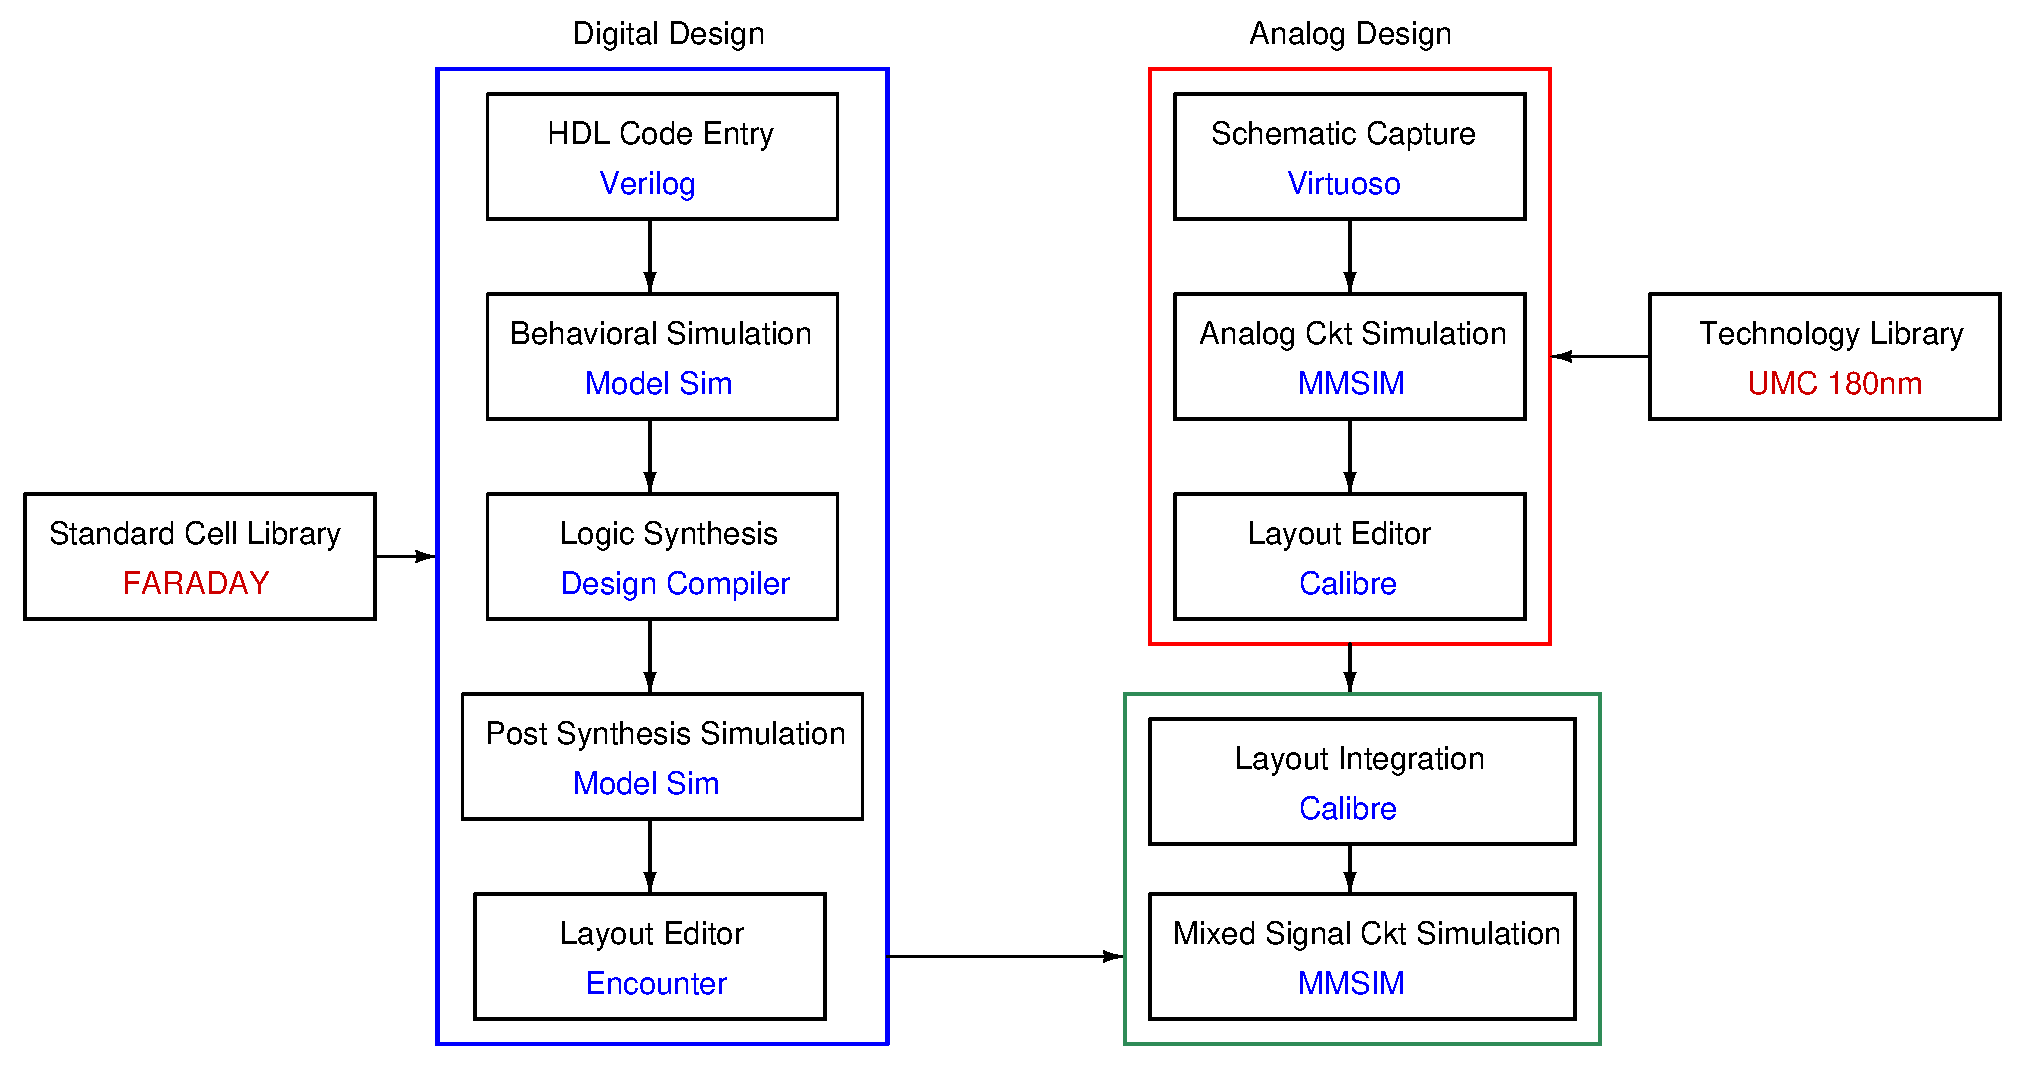
\includegraphics[scale=0.4]{./Figures/MixedSignalDesignFlow.ps}
		\caption{Mixed-Signal Design Flow used in this work}
		\label{fig:FCC}
	\end{center}
\end{figure}


















